\documentclass{beamer}


\usepackage[spanish]{babel} 
\usepackage[utf8]{inputenc} 
\usepackage{amsmath}
\usepackage{hyperref}
\usepackage[nodayofweek]{datetime}
\usepackage{pgfpages}

\usepackage{caption}
\usepackage{subcaption}


\makeatletter
\def\verbatim@font{\ttfamily\tiny}
\makeatother

%~ \usetheme{Berkeley}
\usetheme{CambridgeUS} %~ Ok
\setbeamerfont{frametitle}{size=\small}
%~ \usecolortheme{dolphin}
%~ \usecolortheme{dove}
%~ \usecolortheme{default}
\usecolortheme{seahorse}
%~ \usecolortheme{whale}


%~ \usetheme{Frankfurt}
%~ \usetheme{Madrid}
%~ \usetheme{Malmoe}

%~ \setbeamercovered{transparent}

\logo{%
	   
\includegraphics[scale=.2]{img/logo_ibr.png}
   }
\title[]{Estudios sobre la regulación de la expresión génica por microARNs en plantas mediante estrategias bioinformáticas}

\author{Uciel Chorostecki}
\institute[IBR]{ \\Director Dr. Javier Palatnik\\Instituto Biología Molecular y Celular Rosario}
\date{}

\begin{document}

\frame{\titlepage}

\section{Introducción}

\begin{frame}{miARNs}
    \begin{itemize}
        \item Los microARNs (miARNs) son ARN pequeños de 20-22 nt que regulan la expresión génica en animales y plantas. 
        \item En plantas controlan procesos vitales como el desarrollo, señalización hormonal y respuestas al estrés
    \end{itemize}
\end{frame}

\section{Objetivos}

\begin{frame}{Objetivos}
    \setbeamercovered{transparent=25}
    \pause
	\begin{enumerate}
        \item<1-> Identificar genes regulados por miARNs en plantas.
        \item<-1> Estudiar la biogénesis de los miARNs en plantas.
	\end{enumerate}
\end{frame}

\begin{frame}{Objetivos específicos}
    \setbeamercovered{transparent=25}
		\pause
		\begin{itemize}
            \item<-2> Diseñar una estrategia para la identificación de genes blanco regulados por miARNs en plantas, basado en la conservación evolutiva del par miARN-gen blanco.
            %~ \item<-1> Desarrollar una herramienta web para la predicción de genes blanco de miARNs en diferentes especies de plantas.		
			\item<-1> Desarrollar herramientas que permitan el análisis de los intermediarios de procesamiento de miARNs en plantas a partir de bibliotecas de secuenciación masiva de ARN.
			\item<-1> Identificar y caracterizar precursores de miARNs en distintas especies que tengan mecanismos de procesamiento distintos.
			\item<-1> Caracterizar la relación entre la evolución de los precursores de miARNs en plantas y los mecanismos de procesamiento determinados previamente.
        \end{itemize}
\end{frame}


\section{Resultados}

\subsection{Resultados 1}

\begin{frame}{Aplicaciones bioinformáticas para el estudio de interacciones miARN-gen blanco}
\end{frame}

\begin{frame}{Conservación y divergencia de miARNs en distintas especies}
	\begin{center}
		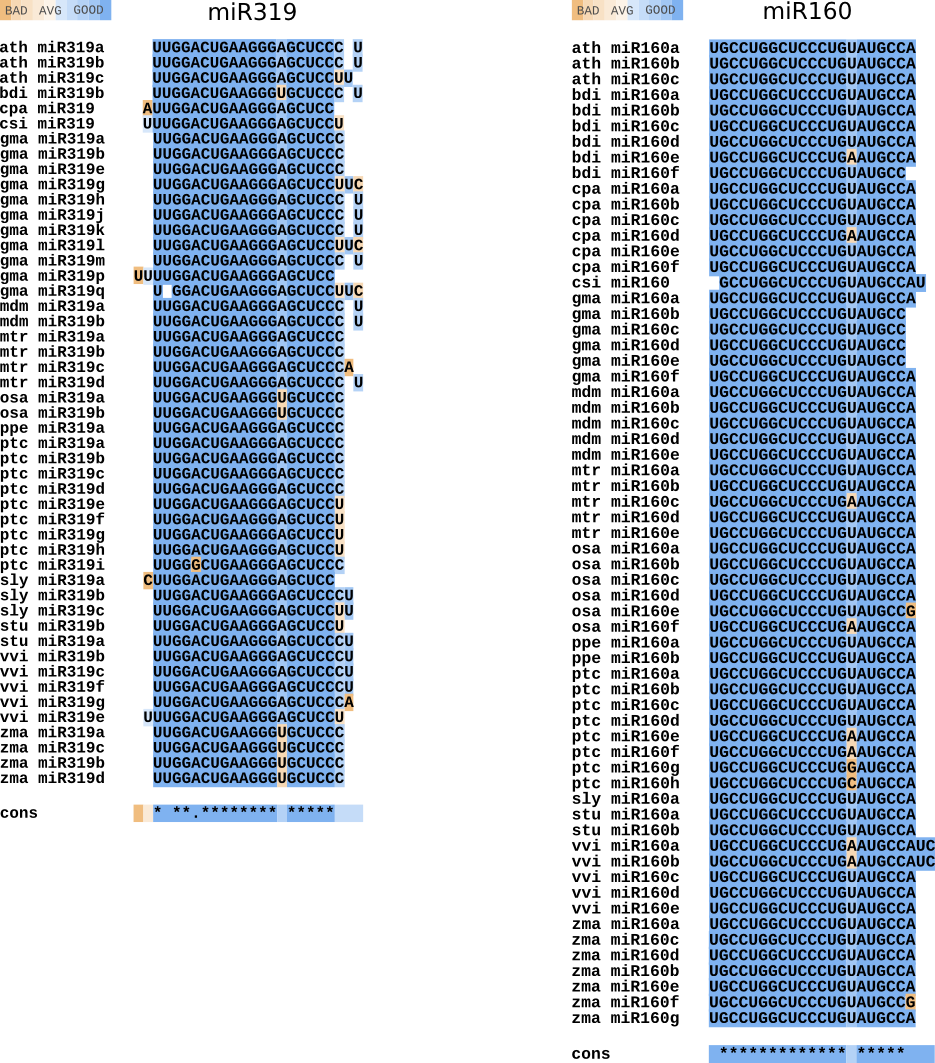
\includegraphics[width=0.5\textwidth]{img/variabilidad_maduro.png}
	\end{center}
\end{frame}

\subsection{Resultados 2}

\subsection{Resultados 3}


\section{Conclusiones}


\begin{frame}{Conclusión I}
	\begin{center}
		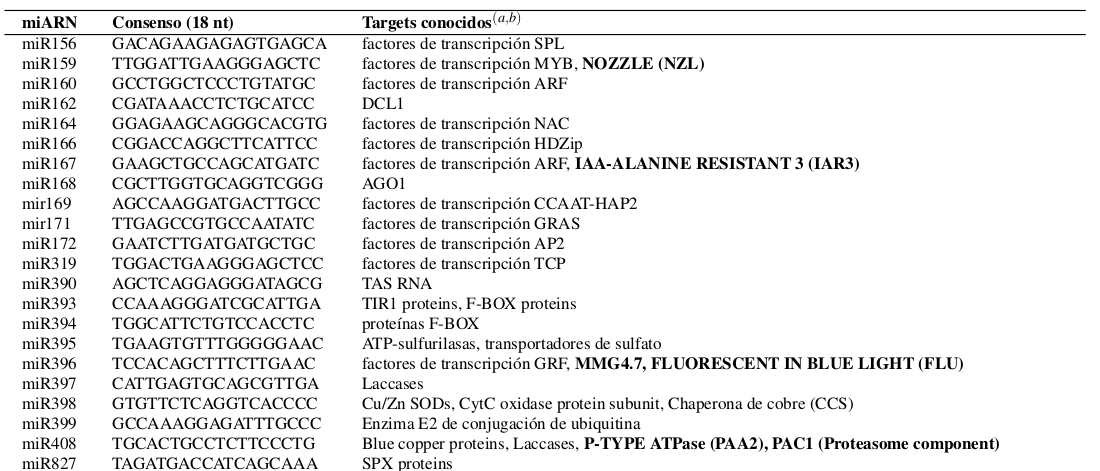
\includegraphics[width=1\textwidth]{img/miRNAs_y_genes_blancos.png}
	\end{center}
\end{frame}

\begin{frame}{Conclusión I}
	\begin{itemize}
        \item<1-> a
        \item<2-> a
        %~ \vspace{1cm}
        \item<3-> a
	\end{itemize}
\end{frame}



\begin{frame}{Objetivos específicos}
    \setbeamercovered{transparent=25}
		\pause
		\begin{itemize}
            \item<-1> Diseñar una estrategia para la identificación de genes blanco regulados por miARNs en plantas, basado en la conservación evolutiva del par miARN-gen blanco.
			\item<-2> Desarrollar herramientas que permitan el análisis de los intermediarios de procesamiento de miARNs en plantas a partir de bibliotecas de secuenciación masiva de ARN.
			\item<-1> Identificar y caracterizar precursores de miARNs en distintas especies que tengan mecanismos de procesamiento distintos.
			\item<-1> Caracterizar la relación entre la evolución de los precursores de miARNs en plantas y los mecanismos de procesamiento determinados previamente.
        \end{itemize}
\end{frame}



\begin{frame}{}
	\begin{center}
		\Huge Muchas gracias.
	\end{center}
\end{frame}

\end{document}
